\documentclass{bioinfo}
\usepackage{hyperref}
%%%%%%%%%%%%%%%%%%%%%% comment boxes

\copyrightyear{2015}
\pubyear{2015}

\begin{document}
\firstpage{1}

\title[BRAKER1]{BRAKER1: Unsupervised RNA-Seq-Based Genome Annotation with GeneMark-ET and AUGUSTUS}
\author[Hoff \textit{et~al}]{Katharina J. Hoff\,$^{1}$\footnote{to whom correspondence should be addressed}, Simone Lange\,$^{1}$, Alexandre Lomsadze\,$^{2}$, Mark Borodovsky\,$^{2,3,4,5}$ and Mario Stanke\,$^1$}
\address{$^{1}$Ernst Moritz Arndt Universit\"{a}t Greifswald, Institute for Mathematics and Computer Science, Walther-Rathenau-Stra\ss{}e 47, 17487 Greifswald, Germany\\
$^{2}$School of Computational Science and Engineering\\
$^{3}$Center for Bioinformatics and Computational Genomics, Georgia Institute of Technology, Atlanta, GA 30332, USA\\
$^{4}$Department of Biological and Medical Physics, Moscow Institute of Physics and Technology, Dolgoprudny, Moscow Region, Russia\\
$^{5}$Joint Georgia Tech and Emory University Wallace H Coulter Department of Biomedical Engineering, Atlanta, GA 30332, USA}

\history{Received on XXXXX; revised on XXXXX; accepted on XXXXX}

\editor{Associate Editor: XXXXXXX}

\maketitle

\begin{abstract}

\section{Motivation:}

GeneMark-ET is a gene prediction tool that incorporates RNA-Seq data into unsupervised training and subsequently generates \textit{ab initio} gene predictions. AUGUSTUS is a gene finder that usually requires supervised training and uses information from RNA-Seq reads in the prediction step.

\section{Results:}
We present BRAKER1, a pipeline for unsupervised RNA-Seq-based genome annotation that combines the advantages of GeneMark-ET and AUGUSTUS. BRAKER1 requires a file with spliced alignments of RNA-Seq reads and a genome file as input. First, GeneMark-ET performs iterative training and generates initial gene structures. Second, AUGUSTUS uses predicted genes for training and then integrates RNA-Seq read information into final gene predictions. In our experiments, we observed that BRAKER1 was more accurate than MAKER2 when it is using RNA-Seq as sole source for training and prediction. BRAKER1 does not require pre-trained parameters or a separate training step.

\section{Availability:}
BRAKER1 is available for download at \url{http://bioinf.uni-greifswald.de/downloads/} and \url{http://exon.gatech.edu/.}.

\section{Contact:} \href{katharina.hoff@uni-greifswald.de}{katharina.hoff@uni-greifswald.de}
\end{abstract}

\section{Introduction}

Transcriptome sequencing data (RNA-Seq) that has been aligned to a genome sequence has great potential to improve the accuracy of structural genome annotation: spliced alignments may indicate intron positions, and coverage increase and decrease may give information about exon-noncoding region borders. Nevertheless, RNA-Seq coverage alone is no reliable indicator of protein coding regions. 

The prediction of protein coding regions in genomes is often accomplished by tools that use statistical models to discriminate genes from other genomic regions. Some of these gene prediction tools can additionally use RNA-Seq alignments to improve prediction accuracy.

The statistical models of gene prediction tools usually require a training  step to adjust parameters to the genomic properties of individual species. For many tools, including AUGUSTUS, the training step has to be performed on an initially existing example gene set. Training gene sets have in the past often been compiled on the basis of expressed sequence tags (ESTs) or protein data, and sometimes have been subject to validation by experts. With the rapidly growing number or novel sequences genomes, this becomes infeasible. Fast and fully automated methods for training gene prediction tools, ideally using the nowadays often available RNA-Seq data, are urgently needed.

In principle, RNA-Seq reads can be assembled into longer contigs, and such contigs can be used similarly to EST data in training of gene finders and for the prediction step. One of the tools that follow this idea is the MAKER2 pipeline [Holt and Yandell, 2011]. However, the RNA-Seq Genome Annotation Assessment Project (RGASP) \cite{RGASP} has shown that transcriptome assembly is prone to errors. To avoid transferring assembly errors into gene prediction, it is therefore advantagous to use the information from unassembled mapped reads.

We have developed BRAKER1, a pipeline that combines the advantages of two gene prediction tools: [TODO: less repetition in this paragraph. be more specific] GeneMark-ET \cite{GeneMark-ET} is a gene prediction tool that incorporates unassembled RNA-Seq reads into unsupervised training and subsequently generates \textit{ab initio} gene predictions.  Genes predicted by GeneMark-ET are subsequently used to train AUGUSTUS \cite{AUGUSTUS}. AUGUSTUS is a gene prediction tool that lacks an unsupervised training procedure but incorporates unassembled RNA-Seq reads into the prediction step; AUGUSTUS was one of the most accurate tools for predicting protein coding genes with RNA-Seq in RGASP. We report accuracy results for BRAKER1 on four model organisms and compare to the accuracy of MAKER2. Recently, Testa et al.~published CodingQuarry, a pipeline for RNA-Seq assembly supported training and gene prediction, but currently recommend its application only to fungi \cite{CodingQuarry}. We compare the results of BRAKER1 on \textit{Schizosaccharomyces pombe} to CodingQuarry.


\begin{methods}
\section{Pipeline Description}

BRAKER1 is implemented in Perl and requires two input files: an RNA-Seq alignment file in \texttt{bam}-format, and a corresponding genome file in \texttt{fasta}-format. Spliced alignment information is extracted from the RNA-Seq file and stored in \texttt{GFF}-format. GeneMark-ET uses the genome file and  the spliced alignment \texttt{GFF}-file for RNA-Seq supported unsupervised training. After training, GeneMark-ET creates an \textit{ab initio} gene set. Those gene structures that have support by RNA-Seq alignments in all introns are selected for automated training of AUGUSTUS. After training, AUGUSTUS predicts genes in the intput genome file using spliced alignment information from RNA-Seq as extrinsic evidence. The pipeline is illustrated in Figure \ref{pipeline}.

\begin{figure}[!tpb]%figure1
\centerline{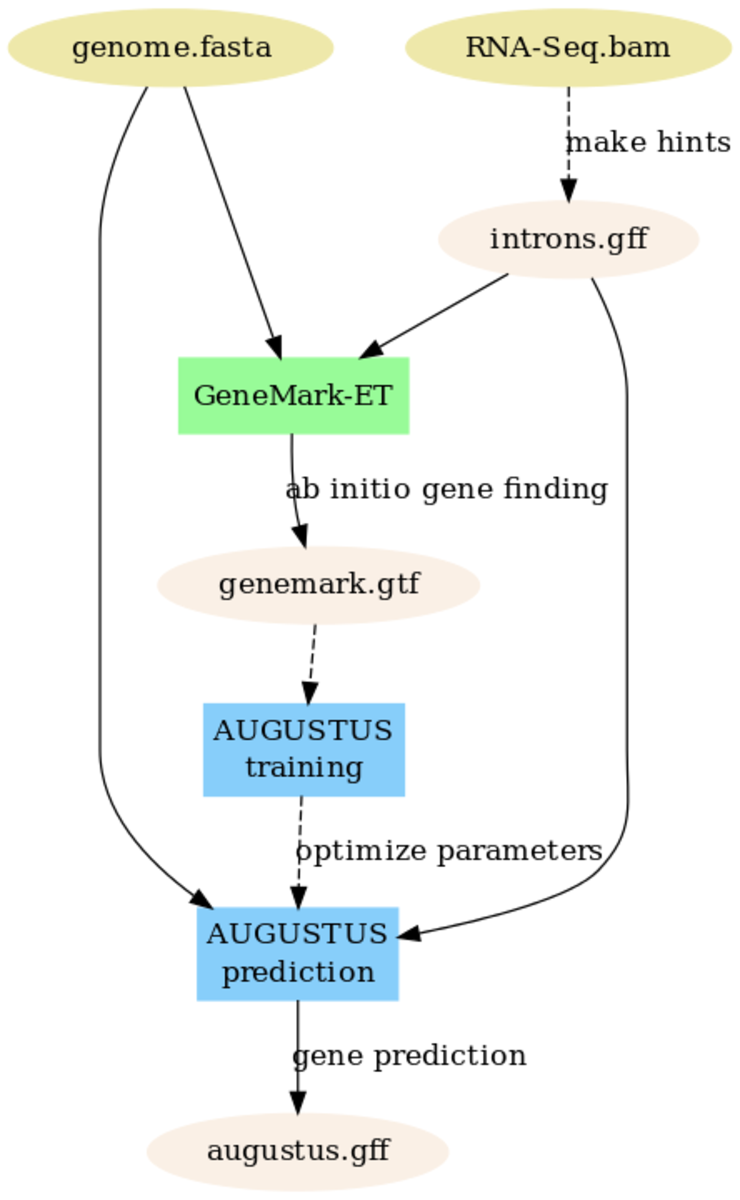
\includegraphics[width=0.6\linewidth]{figs/simple_braker.pdf}}
\caption{Schematic view of the BRAKER1 pipeline.}\label{pipeline}
\end{figure}

\begin{table*}[!b]
\processtable{Accuracy results of BRAKER1 and MAKER2 in genomes of four model organisms. For BRAKER1, accuracy is shown for the GeneMark-ET \textit{ab initio} predictions as well as for the AUGUSTUS predictions with hints from RNA-Seq. For the fungus \textit{S.~pombe}, we also report accuracy results of CodingQuarry.\label{Tab:01}}
{\begin{tabular}{lp{.9cm}p{.9cm}p{.9cm}p{.9cm}p{.9cm}p{.9cm}p{.9cm}p{.9cm}p{.9cm}p{.9cm}p{.9cm}p{.9cm}p{.9cm}}\toprule
 & \multicolumn{3}{c}{\textit{Arabidopsis thaliana}} &  \multicolumn{3}{c}{\textit{Caenorhabditis elegans}} &  \multicolumn{3}{c}{\textit{Drosophila melanogaster}} &  \multicolumn{4}{c}{\textit{Schizosaccharomyces pombe}}\\
 & \tiny{BRAKER1-GeneMarkET} & \tiny{BRAKER1-AUGUSTUS} & \tiny{MAKER2} & \tiny{BRAKER1-GeneMarkET} & \tiny{BRAKER1-AUGUSTUS} & \tiny{MAKER2} & \tiny{BRAKER1-GeneMarkET} & \tiny{BRAKER1-AUGUSTUS} & \tiny{MAKER2} & \tiny{BRAKER1-GeneMarkET} &\tiny{BRAKER1-AUGUSTUS} & \tiny{MAKER2} &\tiny{CodingQuarry}\\
 \midrule
Gene sensitivity & 53.9 & 63.2 & 51.3 & 43.0 & 55.1& 41.0 & 58.5& 70.2 & 58.0 & 80.0& 77.3  & 42.7 & 79.7\\
Gene specificity & 46.1 & 51.3 & 52.5& 41.7& 56.1& 30.8& 49.9 & 59.0 & 46.9& 84.9& 81.2& 68.6 & 72.6\\
Transcript sensitivity & 45.4 & 53.9 & 43.5& 32.9& 43.2& 31.3& 42.3 &52.0 & 42.3 & 80.0& 77.3& 42.7 & 79.7\\
Transcript specificity & 46.1 & 50.0 & 52.5& 41.7 & 54.0& 30.8 & 49.9 & 57.8 & 47.9 &84.9 & 77.4 & 68.6 & 72.6\\
Exon sensitivity & 81.1 & 83.0 & 76.1& 79.9& 80.9& 69.4 & 68.5& 75.1& 64.9& 85.2 & 84.2 & 50.1 & 79.6\\
Exon specificity & 72.4 & 78.5 & 76.1& 78.2& 85.4& 62.3 & 57.9 & 66.2 & 55.0 & 89.0& 82.6& 71.4 & 81.7\\
\botrule

\end{tabular}}{}
\end{table*}

\section{Test Data}

In order to demonstrate prediction accuracy, genomes, reference annotations and RNA-Seq libraries were retrieved for four model organisms from the respective databases: for \textit{Arabidopsis thaliana}, TAIR 10 from \url{http://arabidopsis.org}; for \textit{Caenorhabditis elegans}, WS240 from \url{http://www.wormbase.org}; for \textit{Drosophila melanogaster}, R5 from \url{http://flybase.org}; for \textit{Schizosaccharomyces pombe}, ASM294v2.23 from \url{http://www.pombase.org}. The following RNA-Seq libraries were retrieved from the short read archive at NCBI: SRR934391 (for \textit{A.~thaliana}); SRR065719 (for \textit{C.~elegans}); SRR023505, SRR023546, SRR023608, SRR026433, SRR027108 (for \textit{D.~melanogaster}); SRR097898-SRR097900, SRR097902, SRR097903,
SRR097905-SRR097909, SRR097912, SRR097915, SRR097917, SRR097921, SRR097922, SRR097925, SRR402833 (for \textit{S.~pombe}).



\end{methods}


\section{Results and Discussion}

Since BRAKER1 uses AUGUSTUS being trained on GeneMark-ET, and since AUGUSTUS incorporates RNA-Seq into the prediction step, we expect to see an increase in accuracy when comparing AUGUSTUS to GeneMark-ET. This is the case for \textit{A.~thaliana}, \textit{C.~elegans} and \textit{D.~melanogaster} (see table \ref{Tab:01}). On the fungus \textit{S.~pombe}, GeneMark-ET is superior to AUGUSTUS in the current version of BRAKER1. This is due to the fact that compared to all other test species, the fungus has fewer introns and many intron-less genes. AUGUSTUS parameters can be adapted to improve prediction accuracy in such species, but we here report results with the BRAKER1 default settings. Table \ref{Tab:01} also shows that Transcript sensitivity and specificity of AUGUSTUS is higher because AUGUSTUS reports alternative tanscripts that are supported by RNA-Seq data. 

For the comparison to MAKER2, we followed the tutorial for training and prediction at 
\url{http://weatherby.genetics.utah.edu/MAKER/wiki/index.php/MAKER_Tutorial_for_GMOD_Online_Training_2014}, details can be found in Supplementary Methods. BRAKER1-AUGUSTUS gains 15 percent points in accuracy on gene level when compared to MAKER2. 

On \textit{S.~pombe}, BRAKER1-AUGUSTUS is on average $\sim$4\% more accurate on gene level than CodingQuarry. Notably, GeneMark-ET is even more accurate on this species (when BRAKER1 is used with standard parameters).

BRAKER1 required $\sim$24 hours on a single CPU for training and prediction on \textit{D.~melanogaster}.
[but can be run in parallel?]

\section{Conclusion}

BRAKER1 is a pipeline for training and prediction with the gene finders GeneMark-ET and AUGUSTUS and RNA-Seq data. In contrast to MAKER2, BRAKER1 is a ``one step process'', meaning that after starting it once, it will execute training and prediction without the need for manual command execution. BRAKER1 predicts genes more accurately than MAKER2 and CodingQuarry.

\section*{Acknowledgement}

We would like to thank Mark Yandell and Carson Holt for valuable advice on running MAKER2.

\paragraph{Funding\textcolon} This work is supported by the US National Institutes of Health grant HG000783.

%\bibliographystyle{natbib}
%\bibliographystyle{achemnat}
%\bibliographystyle{plainnat}
%\bibliographystyle{abbrv}
%\bibliographystyle{bioinformatics}
%
%\bibliographystyle{plain}
%
%\bibliography{Document}


\begin{thebibliography}{}
\bibitem[Steijger {\it et~al}., 2013]{RGASP} Steijger,T. and Abril,J.F. and Engstr\"{o}m,P.G. and Kokocinski,F. and The RGASP Consortium, Hubard,T.J. and Guigo,R. and Harrow, J. and Bertone, P. (2013) Assessment of transcript reconstruction methods for
 RNA-seq, {\it Nature Methods}, doi:10.1038/nmeth.271.

\bibitem[Lomsadze {\it et~al}., 2014]{GeneMark-ET} Lomsadze, A. and Burns, P.D. and Borodovsky, M. (2014) Integration of mapped RNA-Seq reads into automatic training of eukaryotic gene finding algorithm, {\it Nucleic Acids Research}, doi:10.1093/nar/gku557.

\bibitem[Stanke \textit{et~al}., 2008]{AUGUSTUS}
Stanke, M. and Diekhans, M. and Baertsch, R. and Haussler, D. (2008) Using native and syntenically mapped cDNA alignments to improve de novo gene finding, \textit{Bioinformatics}, \textbf{24}(5), 637.

\bibitem[Holt and Yandell, 2011]{MAKER2} Holt, C. and Yandell, M. (2011) MAKER2: an annotation pipeline and genome-database management tool for second-generation genome projects, \textit{BMC Bioinformatics}, \textbf{12}:491.

\bibitem[Testa \textit{et~al}., 2015]{CodingQuarry} Testa, A.C. and Hane, J.K. and Ellwood, S.R. and Oliver R.P. (2015) CodingQuarry: highly accurate hidden Markov model gene prediction in fungal genomes using RNA-seq transcripts, \textit{BMC Genomics} \textbf{16}:170.

%\bibitem[Haas \textit{et~al}., 2008] Haas, B. and Salzberg, S. and Zhu, W. and Pertea, M. and Allen, J. and Orvis, J. and White, O. and Buell, C.R. and Wortman, J. (2008) Automated eukaryotic gene structure annotation using EvidenceModeler and the program to assemble spliced reads, {\it Genome Biology}, \textbf{9}(1):R7.

%\bibitem[Keller \textit{et~al}., 2008] Keller, O. and Odronitz, F. and Stanke, M. and Kollmar, M. and Waack, S. (2008) Scipio: Using protein sequences to determine the precise exon/intron structures of genes and their orthologs in closely related species, {\it BMC Bioinformatics}, \textbf{9}(1):278.

\end{thebibliography}
\end{document}
